\section{Test case}
\subsection{Matrices}
Matrices are very important...
Number of non-zero determine matrix size.
Number or row determine problem size.


\begin{tabular}{|r|c|c|c|}
        \hline
        Matrix name & test & test & test\\
        \hline
        Generate & a & b & c\\
        \hline
        SPE10 & a & b & c\\
        \hline
\end{tabular}

\subsection{Code part}
\subsubsection{Factorization}
\subsubsection{Triangular Solve}
\subsubsection{SpMV}


\section{Machines overview}
I used different machines


\subsection{Rostand}
Rostand is a cluster

%   (-_-)   %
\begin{figure}[!ht]
        \centering
        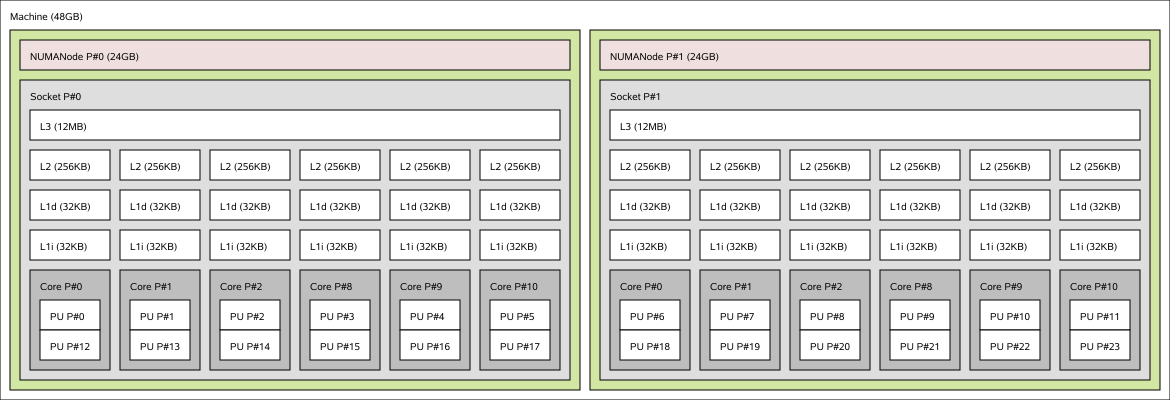
\includegraphics[width=\textwidth]{rostand_lstopo}
        \caption{Architecture of one node of Rostand cluster}
        \label{fig:rostand_lstopo}
\end{figure}

\subsection{Minautore}
Minautore is a cluster of plafrim with 20 numa bank

\section{Results}

To evaluate the benefit of our work we present some experiments on the parallelization of an iterative solver for sparse linear systems.
A popular approach to solve large sparse linear systems of equations is a Krylov method (such as GMRES or Conjugate Gradient) preconditioned by an incomplete factorization (see~\cite{Saad96IMSLS}).
This is often the most time consuming part of a numerical simulation.
The usual way to parallelize this kind of solvers is to use a weaker form of the preconditioner in parallel by preconditioning subdiagonal blocks of the matrix: The subdiagonal blocks are usually obtained thank to a partition of the adjacency graph of the matrix.
Outside the preconditioner, the operations required in a Krylov method are vector operations (mostly BLAS1 type like dot products or AXPY) and matrix vector products.
Those operations are naturally dealt with parallel loop splitting  (e.g., {\em parallel for} in OpenMP).
In this paper, we have chosen to focus on the fine grain parallelization of the ILU preconditioner.
In this case, more levels of parallelism can be obtained because the factorization
and triangular solves of a submatrix can be parallelized on several cores.
Incomplete factorization and associated triangular solve of a sparse matrix
is a problem that is well representative of the difficulty that one can encounter
with fine-grain parallelization: The fine grain description of these algorithms
is natural. However, in practice a straight task based parallelization using TBB or
OpenMP does not deliver good speed-ups because of the very low computational cost of
a task and the NUMA effect when accessing the coefficients of the matrix and vector.
In the experiment results, we will evaluate our programming model on those algorithms.
%% \begin{table}[!h]
%%   \renewcommand{\arraystretch}{1.3}
%%   \caption{Results on the ILU(k) factorization step on a single 4-core
%%     socket with TBB with natural ordering.}
%%   \label{tab:tbb:4:facto:no}
%%   \centering
%%   \begin{tabular}{|c|c||c|c|c|c|}
%%     \hline
%%     Matrix & ILU & Sequential & No agg. & F(32) & CD(4)\\
%%     &     &  (second)  & \multicolumn{3}{c|}{(speed-up)}\\
%%     \hline
%%     \hline
%%     \hline
%%     & ILU(0) & 0.056 & 0.20 & 1.06 & 2.23\\
%%     CUBE\_100 & ILU(1) & 0.142 & 0.46 & 1.54 & 2.81\\
%%     & ILU(2) & 0.611 & 1.30 & 2.58 & {\bf 3.47}\\
%%     \hline
%%     & ILU(0) & 0.262 & 0.65 & 1.89 & 3.09\\
%%     SPE10     & ILU(1) & 0.721 & 1.39 & 2.30 & 3.22\\
%%     & ILU(2) & 1.936 & 1.87 & 2.19 & 3.32\\
%%     \hline
%%   \end{tabular}
%% \end{table}

%-------------------------------
\subsection{Aggregation Overhead}
This section evaluates the overhead caused by the task aggregation
step for several aggregation algorithm instances. As mentioned in
the test description above, the fine-grain DAG generated from the
test cases amount to about 1 million nodes for each matrix. The
number of edges increases when the parameter $k$ of ILU(k) preconditioner increases (see Table~\ref{tab:edges}).
This aggregation step is performed only once for each matrix. Then, the
coarsened DAG is reused as long as the sparse pattern of the matrix is unchanged.
In classical numerical simulation, the mesh on which the equations are discretized
does not change through the simulation, only the coefficients of the linear system
are changing: This means that the aggregation step is typically done only once
while the factorization and triangular solves are called a large number of times (several thousand of times).
The time spent in the task aggregation (Table~\ref{agg_time}) is then usually negligible
compared to the time spent in the factorizations and triangular solves.


On average, applying {\em CD(4)} Coarse String takes 1.5\,s on a DAG with 1 million
of nodes and applying {\em D(400)} takes 3.5\,s.

For {\em CD(4)} aggregation we won on average 0.22\,s per factorization
and 0.31\,s per triangular solve compared to not doing aggregation. So
after only 3 combinations of factorization and triangular solve, the aggregation
become profitable.

For {\em D(400)} aggregation we won in average 0.28\,s per factorization
and 0.49\,s per triangular solve. So after only 5 combinations of factorization
and triangular solve, the aggregation becomes profitable.
% ST: TODO: et donc comparer ce coût par rapport à n fois le gain
% obtenus à chaque phase.

\begin{table}[!h]
  \renewcommand{\arraystretch}{1.3}
  \caption{Aggregation overhead.}
  \label{agg_time}
  \centering
  \begin{tabular}{|c|c||c|c|c|c|}
    \hline
    Matrix & ILU & F(32) & D(400) & CD(4)\\
    &     &  \multicolumn{3}{c|}{(second)}\\
    \hline
    \hline
    \hline
    CUBE\_100  & ILU(0) & 1.534 & 2.945 & 0.908\\
    No         & ILU(1) & 1.467 & 3.032 & 1.119\\
    ordering   & ILU(2) & 1.871 & 3.705 & 1.315\\
    \hline
    CUBE\_100  & ILU(0) & 1.208 & 2.330 & N/A\\
    Nested     & ILU(1) & 2.194 & 3.224 & N/A\\
    dissection & ILU(2) & 3.182 & 3.554 & N/A\\
    \hline
    \hline
    SPE10      & ILU(0) & 1.519 & 3.239 & 1.217\\
    no         & ILU(1) & 1.542 & 3.344 & 1.527\\
    ordering   & ILU(2) & 2.019 & 4.042 & 1.918\\
    \hline
    SPE10      & ILU(0) & 1.292 & 2.541 & N/A\\
    Nested     & ILU(1) & 2.337 & 3.518 & N/A\\
    dissection & ILU(2) & 3.119 & 3.816 & N/A\\
    \hline
  \end{tabular}
\end{table}
